\documentclass[11pt]{article}
\usepackage{amsmath,amssymb,amsthm,amsfonts}
\usepackage{graphics}
\usepackage{graphicx,epsfig,epstopdf}
\usepackage{natbib, amsmath, mathtools}
\usepackage[hmargin=1in,vmargin=1in]{geometry}

\newcommand{\new}[1]{\textcolor{blue}{{#1}}}

\begin{document}

The elastic flexure system shown in Figure \ref{fig_2005_002}(a) is designed to allow the right bar to move vertically. %without changing its angular orientation.
Both flexures are of length $L$, and uniform thickness $h$ and a
width $b$ (into the plane of the paper). The material of each
flexure has a Young's Modulus, $E$.

\begin{figure}[h!]
\centering
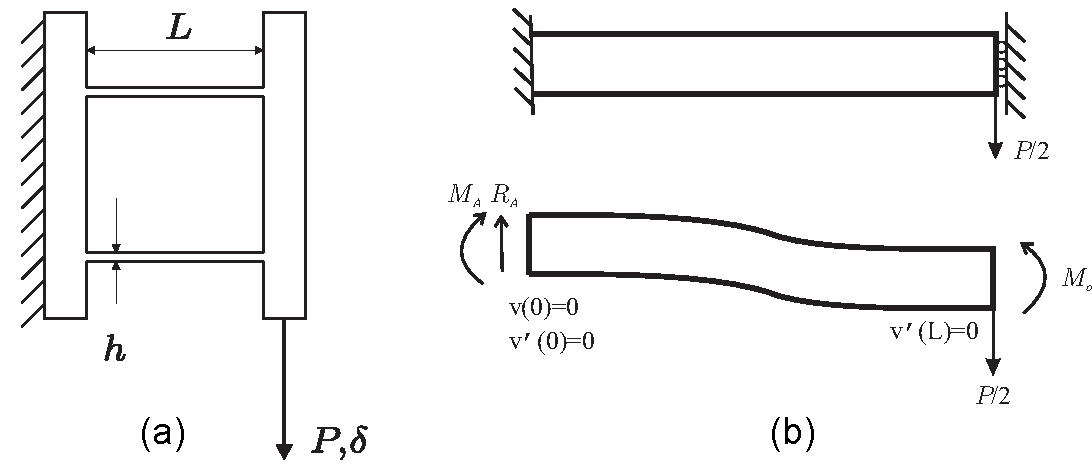
\includegraphics[width=0.7\textwidth]{Flexure_structure_with_hints}
\caption{(a) Flexure structure. (b)  A free body diagram of one flexure.}
\label{fig_2005_002}
\end{figure}

\begin{enumerate}

\item Derive an expression for the  stiffness $k= {P}/{\delta}$ of the flexure
system.

\textbf{Hint:} {\em From the symmetry of the structure (the two flexures have the same material, geometry, and boundary conditions), we can simplify the problem by equivalently considering each flexure acted upon by an applied load $P/2$. Because the two are rigidly connected, each one will have the same deflection. A free body diagram of one flexure is shown in Figure \ref{fig_2005_002}(b). You are essentially required to find the tip deflection, $\delta = v(L)$, in Figure \ref{fig_2005_002}(b).}

\item Plastic deformation in the flexure occurs when the
maximum stress in the flexure reaches the tensile yield strength,
$\sigma_y$. In terms of the geometric parameters $\left\{L,h,b\right\}$ and the
material properties $\{ E, \sigma_y\}$, determine the maximum
deflection $\delta_{max}$ which can be obtained without causing any
plastic deformation in the flexures.

\item For $L=50$\,mm, $h=1.5$\,mm, $b=6$\,mm, $E=100$\, GPa and
$\sigma_y=350$\,MPa (phosphor bronze), what is $\delta_{max}$?
\end{enumerate}

\end{document}
